

\begin{frame}[fragile]{Lineage specific evolution}
   \begin{columns}[T,onlytextwidth]
    \column{0.5\textwidth}
    \begin{figure}
		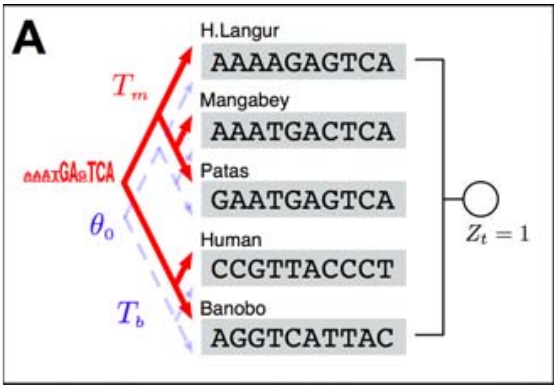
\includegraphics[width=0.77\textwidth]{images/monkey-model.png}
        \caption{Modeling full phylogeny as one component}
	\end{figure}
    \column{0.5\textwidth}
    \uncover<2>{\begin{figure}
		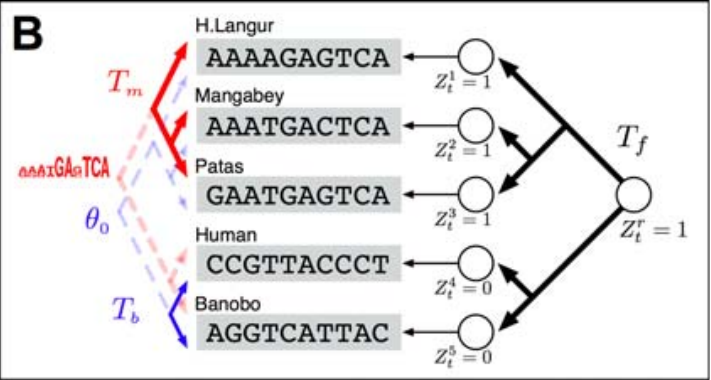
\includegraphics[width=\textwidth]{images/csmet-model.png}
        \caption{Modeling full phylogeny as one component}
	\end{figure}}
    \end{columns}
\end{frame}

\begin{frame}[fragile]{Ornstein-Uhlenbeck Models: Whole TFBS evolving as a unit}
\begin{itemize}
\item HB models neglects lineage or specie specific selection
\item OU models this gap by accounting for lineage/specie specific selection by requiring regime specific optima to be obtained
\item OU models can account for whole element substituion by defining a quantitative trait as a score attached to the TFBS $X(t)$
\item $X(t)$ evolves by two components one deterministic, other stochastic (BM)
\end{itemize}
\begin{align*}
dX(t) &= \alpha(\theta-X(t)) + \sigma dB(t)\\
\alpha & = \text{Strength of selection}\\
\theta - X(t) & = \text{Distance from optimum value}\\
\sigma &= \text{strength of random drift}\\
dB(t) &= \text{random white noise}
\end{align*}
\end{frame}




\section{Brownian Motion and Evolution}


\begin{frame}[fragile]{Ornstein-Uhlenbeck Models: Whole TFBS evolving as a unit}
   \begin{columns}[T,onlytextwidth]
    \column{0.3\textwidth}
	\begin{figure}
    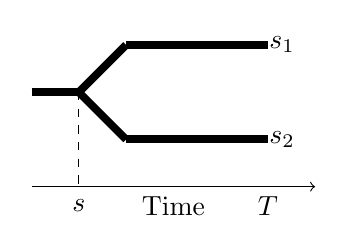
\begin{tikzpicture}[scale=0.6]
    \tikzstyle{operator} = [draw,fill=white,minimum size=1em] 
        \draw[->] (0,-2) -- (6,-2);
        \draw[line width=1mm] (0,0) -- (1,0);   
        \draw[line width=1mm] (1,0) -- (2,1);
        \draw[line width=1mm] (2,1) -- (5,1);
        \draw[line width=1mm] (1,0) -- (2,-1);
        \draw[line width=1mm] (2,-1) -- (5,-1);   
        \draw[dashed] (1,0) -- (1,-2);
        \node at (1,-2.4) {$s$};
        \node at (3,-2.4) {Time};
        \node at (5,-2.4) {$T$};
        \node at (5.3,1) {$s_1$};
        \node at (5.3,-1) {$s_2$};
    \end{tikzpicture}
\caption{$s_1$, $s_2$ -- BM}    
\end{figure}

	\column{0.7\textwidth}    
    \begin{align*}
E[\mathbf{X}(t)] &= \begin{pmatrix}
\theta_0\\
\theta_1
\end{pmatrix}\\
 \texorpdfstring{{\Sigma}} &= \sigma^2\begin{pmatrix}
T & s\\
s & T
\end{pmatrix}\\
\end{align*}    
  \end{columns}
  \begin{columns}[T,onlytextwidth]
    \column{0.3\textwidth}     
    \begin{figure}
    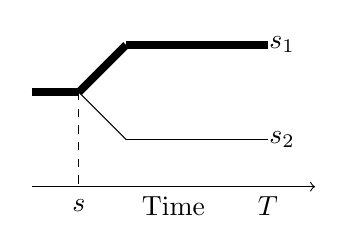
\begin{tikzpicture}[scale=0.6]
    \tikzstyle{operator} = [draw,fill=white,minimum size=1em] 
        \draw[->] (0,-2) -- (6,-2);
        \draw[line width=1mm] (0,0) -- (1,0);   
        \draw[line width=1mm] (1,0) -- (2,1);
        \draw[line width=1mm] (2,1) -- (5,1);
        \draw (1,0) -- (2,-1);
        \draw (2,-1) -- (5,-1);   
        \draw[dashed] (1,0) -- (1,-2);
        \node at (1,-2.4) {$s$};
        \node at (3,-2.4) {Time};
        \node at (5,-2.4) {$T$};
        \node at (5.3,1) {$s_1$};
        \node at (5.3,-1) {$s_2$};
    \end{tikzpicture}
    \caption{$s_2$ -- new optimum regime, $s_1$ -- ancestral}    
\end{figure}
    \column{0.7\textwidth}
    \begin{align*}
      E[X_1(T)] &= \theta_0e^{-\alpha T}+ \theta_1(1-e^{-\alpha T})\\
      E[X_2(T)] &= \theta_0e^{-\alpha T} + \theta_1e^{-\alpha(T-s)}(1-e^{-\alpha s})\\ 
      &+ \theta_2(1-e^{-\alpha(T-s)})\
	\end{align*}
  \end{columns}
\end{frame}
